\documentclass[journal]{IEEEtran}

\ifCLASSINFOpdf
  % \usepackage[pdftex]{graphicx}
  % declare the path(s) where your graphic files are
  % \graphicspath{{../pdf/}{../jpeg/}}
  % and their extensions so you won't have to specify these with
  % every instance of \includegraphics
  % \DeclareGraphicsExtensions{.pdf,.jpeg,.png}
\else
  % or other class option (dvipsone, dvipdf, if not using dvips). graphicx
  % will default to the driver specified in the system graphics.cfg if no
  % driver is specified.
  % \usepackage[dvips]{graphicx}
  % declare the path(s) where your graphic files are
  % \graphicspath{{../eps/}}
  % and their extensions so you won't have to specify these with
  % every instance of \includegraphics
  % \DeclareGraphicsExtensions{.eps}
\fi


\usepackage{url}
\usepackage{graphicx}
\usepackage{subfig}
\usepackage{float}
\usepackage{dblfloatfix}
\usepackage{verbatim}
\usepackage{algorithm}
\usepackage{algorithmic}



% correct bad hyphenation here
\hyphenation{op-tical net-works semi-conduc-tor}


\begin{document}
%
% paper title
% Titles are generally capitalized except for words such as a, an, and, as,
% at, but, by, for, in, nor, of, on, or, the, to and up, which are usually
% not capitalized unless they are the first or last word of the title.
% Linebreaks \\ can be used within to get better formatting as desired.
% Do not put math or special symbols in the title.
\title{Design Methods for Unmanned Vehicles \\Project Report}
%
%
% author names and IEEE memberships
% note positions of commas and nonbreaking spaces ( ~ ) LaTeX will not break
% a structure at a ~ so this keeps an author's name from being broken across
% two lines.
% use \thanks{} to gain access to the first footnote area
% a separate \thanks must be used for each paragraph as LaTeX2e's \thanks
% was not built to handle multiple paragraphs
%

\author{Matteo~Mastrogiuseppe,~\IEEEmembership{231762}  \\
Daniele~Serafini,~\IEEEmembership{232273}
        }% <-this % stops a space



% make the title area
\maketitle

% As a general rule, do not put math, special symbols or citations
% in the abstract or keywords.
\begin{abstract}
Exploration and mapping are fundamental tasks in the field of robotics, with applications ranging from autonomous navigation to search and rescue. This paper proposes a framework capable of achieving a fully autonomous exploration and mapping, by deploying multiple robots equipped with RGB-D cameras.
Our system incorporates real-time sensor fusion techniques to create detailed and up-to-date 3D maps of the environment. Furthermore, we propose a multi-robot coordination algorithm that enhances the efficiency of exploration while promoting the coverage of larger unknown areas. Our work also enhances path planning by integrating A* with artificial potential fields derived from Fast Marching Method,  effectively considering obstacle avoidance and optimality in the exploration process. 
Through simulations, we demonstrate the effectiveness of our multi-robot system in diverse scenarios. Our approach harnesses the full potential of RGB-D cameras to produce high-quality maps while enhancing exploration efficiency. 
\end{abstract}


% For peer review papers, you can put extra information on the cover
% page as needed:
% \ifCLASSOPTIONpeerreview
% \begin{center} \bfseries EDICS Category: 3-BBND \end{center}
% \fi
%
% For peerreview papers, this IEEEtran command inserts a page break and
% creates the second title. It will be ignored for other modes.
\IEEEpeerreviewmaketitle

\section{Introduction}
% ========================================= %
%\subsection{Context of the work. Scenarios where the project can be used. Open challenges and issues}
Exploration and mapping of unknown environments constitute core tasks in the field of robotics, with profound implications across various domains. Applications range from autonomous driving to search and rescue missions, from inspection in confined spaces to industrial automation tasks demanding spatial awareness. In these applications, the ability to generate accurate and comprehensive maps of the environment is key for the success of robotic systems. The evolution of sensor technologies and algorithms has led to the development of very sophisticated solutions to the Simultaneous Localization and Mapping (SLAM) problem. This has empowered these robotic systems to navigate, perceive, and map complex and dynamic environments with remarkable precision. 

The incorporation of RGB-D cameras, capable of capturing both color and depth information, represents a pivotal advancement in providing robots with sophisticated perception capabilities. Their ability to provide rich, three-dimensional data in real-time has opened up new possibilities for improving the quality and efficiency of mapping tasks. 

While single-robot exploration and mapping using RGB-D sensors have shown great results, the scalability and effectiveness of such systems can be significantly enhanced through the collaboration of multiple robots. The possibility to deploy multiple robots with capabilities of self localization and mapping allows to store single portions of map that are computationally lighter and that can be manipulated and merged in post production.

Despite remarkable advancements, several challenges and open issues persist in this domain. The fusion of RGB-D sensors to construct accurate point clouds and 3D maps remains a complex task, demanding real-time processing capabilities and robust algorithms to handle varying environmental conditions. The collaborative aspect of multi-robot systems introduces coordination challenges, where robots must work synergistically, share information, and avoid conflicts to achieve their common objectives. Exploration strategies necessitate refinement to optimize resource allocation, reduce redundancy, and ensure comprehensive coverage of unknown terrains. Path planning algorithms need to strike a balance between efficiency and safety, drawing routes that circumvent obstacles while minimizing travelling times.


% ========================================= %
%\subsection{Possible solutions, new technology, recent innovations. Introduce work done and goals}
Recent approaches to visual SLAM are deploying direct visual motion methods or feature-based methods \cite{macario2022comprehensive}. The latter typically extract and track distinct features, such as keypoints or corners, from images and use the relative motion of these features to estimate the camera pose. Direct visual motion methods do not rely on distinct feature points, but instead operate directly on the raw pixel intensities of the images. 
For what concerns the exploration task, different strategies for robot swarms have been proposed, aiming at full autonomy in the process. Techniques such as distributed mapping, where robots share and fuse local maps, and frontier-based exploration, guiding robots to unexplored regions, enhance efficiency and adaptability. 
At the same time, contemporary path planning strategies for robots leverage advanced techniques like sampling-based methods, bionic algorithms, and artificial potential fields. These approaches optimize obstacle avoidance and allow the robot to adapt to dynamic environments.
Additionally, the integration of artificial intelligence and machine learning techniques holds the promise of enhancing the general adaptability and autonomy of these robotic systems, in all of their aspects.


In this context, our research introduces a general framework which aims at achieving complete autonomous exploration and mapping, using multiple robots each equipped with an RGB-D camera. This is achieved by investigating the problem in its sub-challenges: SLAM solution and point cloud handling, multi-robot exploration strategy, and path planning.
We explore latest frontiers in point cloud processing, incorporating state-of-the-art algorithms to ensure accurate map merging. Refined exploration strategies are discussed, using frontier-based approaches to intelligently guide multi-robot teams. Path planning is enhanced through the integration of artificial potential fields derived from Fast Marching Methods (FMM) to the general A*, ensuring both obstacle avoidance and optimality.


% ========================================= %
%\subsection{Contributions, as a list}
The main contributions of this work can be outlined as follows:
\begin{itemize}
    \item Formalizing a global strategy to use in multi-robot exploration, using RGB-D sensors. The goal is to cover the main, relevant problematics associated with the task, analyze them, and propose a suitable combination of methods and techniques.
    \item Deploying the state-of-the-art RTAB-Map software to multiple robots and merging the final maps and point clouds. In this way, the solution of the SLAM problem is decentralized, and it is easier to tackle more complex environments.
    \item Investigating a strategy to autonomously explore an unknown environment with multiple robots, making sure that the agents are coordinated and effectively distributed.
    \item Proposing a path planning algorithm which combines graph search methods with artificial potential fields, ensuring collision avoidance and efficient trajectories.
\end{itemize}
% ========================================= %
%\subsection{Report Organization}
The rest of the report is organized as follows. Related work is reviewed in Section \ref{sec:literature}. Section \ref{sec:methods} discusses the methodology used in this project work. All aspects of the proposed framework are described, and the reasoning behind the adoption of the techniques is explained. Simulation results are presented in Section \ref{sec:results} and the effectivness of our framework is shown. Finally, conclusions are drawn in Section \ref{sec:conclusion}, along with a brief discussion of the limitations of the present work and possibilities for further implementations.



% ========================================= %

%with algorithms like Iterative Closest Point (ICP) and truncated-ICP (trICP), taking in consideration both the translation and rotations between the maps obtained. 
%Nonetheless, building a fast, real time, SLAM and point-cloud reconstructor framework using an RGB-D camera and ICP-like algorithms is a challenging task, because it requires a high computational effort to obtain translations and rotations directly form the recorded point clouds.

%Given these difficulties, the approaches to visual SLAM present in literature are deploying direct visual motion methods or feature-based methods \cite{macario2022comprehensive}. Direct visual motion methods work with the raw image intensities and directly optimize for the camera pose and the scene geometry. They do not rely on distinct feature points, but instead operate directly on the raw pixel intensities of the images. Feature based methods typically extract and track distinct features (such as keypoints or corners) from images and use the relative motion of these features to estimate the camera pose. 
%RGB-D based SLAM excels when the environment is large and rich in terms of features to be tracked for loop closures. 
%Loop closure is a pivotal process in SLAM using visual RGB-D mapping. It plays a critical role in maintaining the accuracy of robot trajectories and maps by recognizing when the robot revisits previously explored locations and correcting any accumulated errors in pose estimation and mapping. To achieve loop closure, distinctive visual features are extracted from RGB-D images captured by the sensor. These features are then compared to past observations to identify potential matches. Geometric verification techniques are used to confirm loop closure by estimating the transformation between current and past observations. If this transformation meets predefined criteria, a loop closure is declared, ensuring accurate SLAM performance for three-dimensional modeling in real-time with low sensor cost utilization. Loop closure information is integrated into a graph-based SLAM framework, where optimization algorithms refine the entire map and trajectory for global consistency. This process greatly improves the reliability and accuracy of the mapping system, allowing it to navigate in real-world environments with minimal drift and error accumulation. 

%The loop closure detection becomes no more trivial when this approach is applied to multi-robot exploration and mapping. The ability to create real-time maps of the environment while accurately tracking the position and pose of multiple robots is crucial for various applications to speed up the activity required from the tasks, being it autonomous navigation, surveillance, search and rescue, or collaborative mapping. Multi-Visual Loop closure detection has seen notable progress. The algorithms now employ sophisticated techniques like bag-of-words, global feature descriptors, and deep learning-based methods to identify and close loops in the map, reducing drift errors and enhancing long-term accuracy.




\section{Related Work}
\label{sec:literature}

    

\begin{comment}
Talk about:
\begin{itemize}
    \item We will use the ROS framework. So we need to choose between the available mapping libraries. RTAB-Map is a good fit for our needs, since it reaches state-of-the-art levels of accuracy. Talk about SLAM, visual odometry, dense point cloud reconstruction, say that they are all top level. Most importantly, it also generates a 2D occupancy-grid, like lidar-based algorithms do. Occupancy grids are the starting point of autonomous exploration and navigation algorithms. And so on.
    

\end{itemize}
\end{comment}


\subsection{Multi Visual SLAM}

In multi-robot setups, where data gathering and estimating the robots' positions are distributed among multiple entities, communication between these agents becomes essential. Collaborative SLAM (C-SLAM) and multi-robot systems, in general, involve a critical distinction between two perspectives: global and local. In a global, centralized, approach, the estimator has a comprehensive view of the entire team of robots, making estimations based on perfect knowledge of each robot's measurements. This means it takes into account all the data from all robots collectively \cite{lajoie2021towards}. However, as the number of robots grows, trying to address centralized C-SLAM becomes impractical due to communication limitations. Therefore, a more effective way to handle scalability is by tackling C-SLAM in a decentralized fashion. In this approach, each robot independently creates its own local map and combines some information from other robots, along with measurements taken between robots, to reach a solution that's specific to its immediate surroundings. Through a series of interactions with its neighboring robots, the local solution of each robot gradually aligns with a solution that matches the overall global reference frame. An alternative to this approach is the complete C-SLAM approach adopted for large-scale environments during the DARPA Subterranean Challenge \cite{denniston2022loop}, or the one presented in the COVINS project \cite{schmuck2021covins}. In this kind of approaches the back-end (generating state estimates using all measurements gathered) and front-end (handling perception-related tasks) of C-SLAM do not necessarily occur fully on a single robot anymore depending on the sensing, communication, and estimation strategies. 

Focusing only on the front-end, the one in
charge of producing landmark estimates, odometry measurements, and both intra-robot and
inter-robot loop closures, we can see two distinctive typologies of loop closures: direct and indirect. Direct inter-robot loop closures occur when two robots meet, and they are able to estimate their current relative location with respect to each other through direct sensing. Indirect inter-robot loop closures instead occur when the robots examine their maps to identify areas that they both have explored. By comparing these shared areas, the robots can figure out how they are positioned relative to each other and estimate the transformations needed to align their maps.

In this latter approach, where loop closure detection is basically the extension of single-robot loop closure detection
to multiple maps, there are different visual-based solutions:

\begin{itemize}
    \item \textbf{Visual bags of binary words:} it is based on feature extraction and visual vocabulary as clusters. The main concept is to represent images using binary descriptions, which are highly efficient for tasks that need to be done quickly, like recognizing objects or places in real-time. These descriptions are like digital fingerprints that capture unique visual details in the images, making it easier and faster to find and identify specific locations or scenes \cite{galvez2012bags}.

    \item \textbf{Deep learning:} this method is based on place recognition with deep learning, where fixed-length vector represent each input image. This representation encodes the visual content of the image in a way that is suitable for efficient matching and retrieval and computation through Convolutional Neural Networks: the whole systems is called NetVLAD (Network Vector of Locally Aggregated Descriptors) \cite{arandjelovic2016netvlad}.

\end{itemize}

There are also different methods starting from 3D point clouds:

\begin{itemize}
    \item \textbf{Global point cloud descriptors:} this is a combination of the previously mentioned NetVLAD and the novel  PointNet architecture, designed for processing point cloud data and extraction of meaningful features from unordered point clouds \cite{uy2018pointnetvlad}. 

    \item \textbf{Place recognition:} based also on a ICP algorithm, it focuses on the determination of reduced observability and geometric degeneracy to avoid closing loops in ambiguous areas with high level of geometric degeneracy as it could result in catastrophic distortions of the map. Using this solution, areas with high level of geometric degeneracy that can lead to data association ambiguity and spurious loop closures are removed from loop closure consideration \cite{ebadi2021dare}.

\end{itemize}




\subsection{Exploration Strategy}
\label{sec:literature_exploration}

Given the capability of each robot to independently construct its own map, an exploration strategy must be defined.  This strategy serves as the guiding principle that allows the robot to autonomously navigate and expand its mapped terrain.
The widely adopted and conventional approach is known as frontier-based exploration \cite{frontier_based}. Frontiers denote those spatial regions situated at the interface between explored and uncharted territories. By directing the robot's movement towards these frontiers, it can gain information about new, unexplored regions. Eventually, moving to successive frontiers, the robot will constantly increase its knowledge of the map.

Multi-robot, frontier-based exploration mainly revolves around the the detection of frontiers in the global map and the assignment of these to the individual robots as navigation goals.

Frontiers can be detected using edge detection techniques on the grid-map \cite{frontier_based}. This method capitalizes on the pronounced contrast between pixels, achieving reasonable speed and good accuracy. Filtering out obstacles, it is possible to identify safe regions to be explored. It's worth noting that while this technique is exclusively applicable in 2D environments, this limitation does not impede its utility in our specific context.

Umari and Mukhopadhyay \cite{rrt_exploration} propose the use of Rapidly-exploring Random Trees (RRT) to detect frontiers. As a sampling-based approach, RRT stands out for its exceptional computational efficiency, making it versatile for deployment in 3D environments and its proficiency in addressing path planning challenges. However, for exploration based only on RGB-D cameras, it is crucial that the robot targets the centroid of the unexplored area and that it creates a path which steers outside of the obstacles. This is particularly vital for scenarios where algorithms like RTAB-Map require ample clearance from obstacles to reconstruct an accurate occupancy grid. For this reason, we want to make sure to find a point as far from obstacles as possible, rather than opting for arbitrary points along the edge. Additionally, the path itself should be as smooth as possible and which steers clear from obstacles, a level of performance not readily achieved by employing a straightforward RRT approach.

Efficiently assigning the identified frontiers to individual robots necessitates a strategy that minimizes redundancy and promotes a balanced and effective distribution. Two primary factors come into play here: the formulation of a reward function and the subsequent policy for assignment based on this function. Numerous assignment policies have been proposed \cite{allocation}, but in general, they predominantly rely on the robot-frontier distance as the primary metric. Particularly when dealing with a limited number of robots, the distribution of frontiers among the robot team tends to take precedence over other factors, such as the value function we define.
Consequently, we will introduce a reward function designed to encompass not only the robot-goal distance but also the potential information gain achievable by exploring a specific frontier. In doing so, we aim to strike a balance between robot proximity to frontiers and the value of exploring those frontiers, thus optimizing the allocation of tasks among the robot team.

    
\subsection{Path planning:}
Path planning is a core and widespread problem in robotics. Over the years, a variety of methods have been suggested to address this issue \cite{path_planning_review}. Hereafter, we outline the most commonly employed strategies, highlighting both their principal benefits and limitations.
\begin{itemize}
    \item \textbf{Sampling Based Methods}: they construct a path by randomly sampling points within the configuration space, which represents all possible robot configurations. These sampled points are then connected to form a feasible path. Since they focus solely on the configuration space, they excel in scenarios with numerous motion constraints. Their computational efficiency makes them particularly well-suited for navigating 3D environments or higher-dimensional search spaces.
    Baseline algorithms, such as the RRT algorithm, are capable of finding paths but do not offer optimality guarantees. Enhanced variants like RRT* yield improved results and can, in theory, provide an optimal path with an infinite number of samples \cite{rrt_star}. Generally, they exhibit limited sensitivity to the environment, but their convergence may decelerate significantly in the presence of multiple obstacles..
    \item \textbf{Graph Search Techniques}: these algorithms explore a graph (in this case a grid-map), while taking into account various cost factors and heuristic estimates for cell-to-cell transitions. Prominent examples include the Dijkstra Algorithm and the optimal A* algorithm. They can effectively and reliably find the shortest path in a 2D grid environment. Nevertheless, their computational cost significantly escalate when applied to 3D settings, leading to reduced usage in higher-dimensional spaces.
    \item \textbf{Artificial Potential Field}: typically applied in the context of \textit{local} path planning due to its strong suitability for obstacle avoidance. Notably, for extended trajectories, robots are susceptible to becoming trapped in local minima within the potential field.
    \item \textbf{AI-based Methods}: neural networks find applications also in path planning, as they can implicitly grasp the mapping from perception space to behavioral space. For instance, Deep Q-Learning-based methods have been explored in this context \cite{q_learning}. However, handling vast and intricate environments remains a challenge for neural networks, and a universally ideal neural network architecture for this task has yet to emerge.
    \item \textbf{Bionic Algorithms}: these approaches draw inspiration from the collective behaviors observed in biological swarm intelligence within the natural world. Notable examples include genetic algorithms, ant colony optimization, particle swarm optimization, and the grey wolf optimizer. This category of methods has garnered significant attention in recent research. Nevertheless, they still face a number of drawbacks, such as challenges in scaling to higher-dimensional spaces and susceptibility to the precise tuning of parameters.
\end{itemize}
In specific, in this work we will present a method which fuses the core ideas of Graph Search Algorithms and Artificial Potential Fields.


\section{Project Work}
\label{sec:methods}
% ======================= %
\begin{figure*}[t]
  \begin{center}
    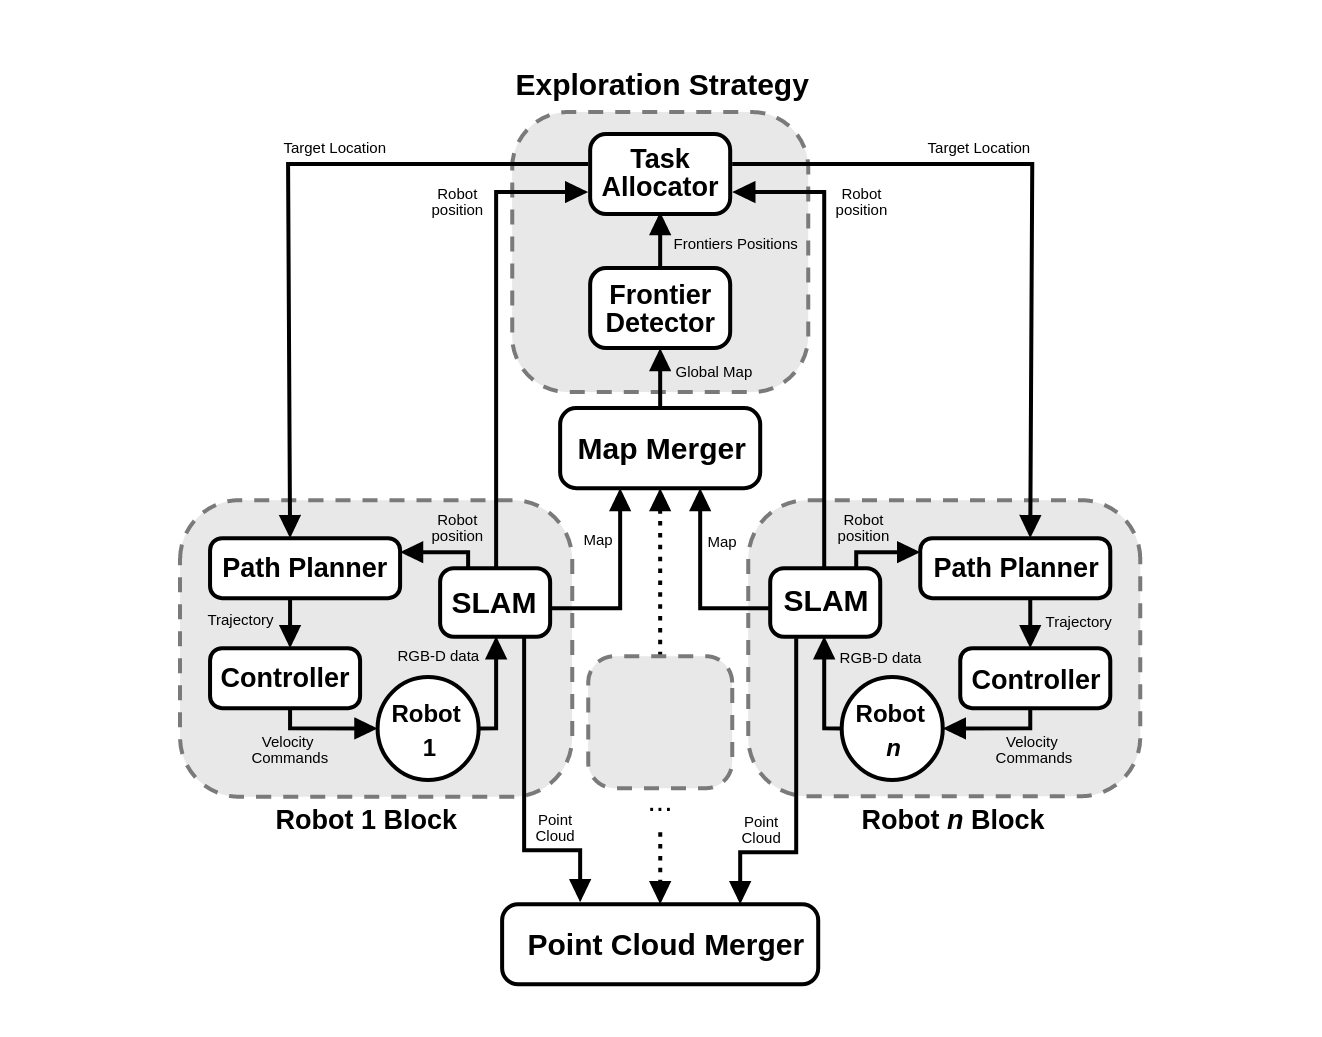
\includegraphics[width=0.7\textwidth]{img/simulation.png}
  \end{center}
  \caption[]{
    \textbf{Simulation Environment.} 
    Scheme of the multi-robot exploration. The maps built by the individual robots are merged to create a global map. Frontiers are detected and assigned to the robots as navigation goals.
  }
  \label{fig:simulation}
\end{figure*}

%
Our project work aims at developing a framework capable of achieving autonomous multi-robot exploration and mapping. Building an efficient, real time, SLAM and point-cloud manager software using an RGB-D camera is a challenging task, because solving the SLAM problem while reconstructing the point clouds requires a high computational effort. The open source Real‐Time Appearance‐Based Map (RTAB-Map) \cite{rtabmap} is the best fit for our needs given its ability to handle dense point cloud reconstruction, hybrid feature-based and graph-based SLAM, as well as the creation of an occupancy grid for navigation purposes. This solution is also focused on a loop closure detection algorithm based on the bag‐of‐words approach, where features can be any of the types included in OpenCV or ORB or more. 

Through this tool, it is possible to create a working framework where all the map-handling functions are fully defined. Therefore, it allowed us to focus on the concepts of exploration, path planning and merging of the individual point clouds. 

\begin{comment}
To do so, we mostly cover three areas: SLAM and mapping, exploration strategy and path planning.

\end{comment}
The general scheme of the simulation model is shown in Figure \ref{fig:simulation}.

\subsection{Feature-based SLAM}

In RTAB-Map distinctive features in RGB-D data  are used to identify and track landmarks or key points in the environment, enabling the robot to create a map and estimate its own position within that map. The main steps to achieve a full map are the following:

\begin{itemize}
    \item \textbf{Feature Extraction}: visual features extraction to perform odometry and loop closure detection
    The first step in this feature-based approach is to extract distinctive features from sensor data. In the case of a camera, these features could be key points like corners or blobs. From this visual data RTAB-Map extracts distinctive visual features from each frame. These features help in identifying and matching keypoints across different frames, facilitating visual odometry and loop closure detection
    
    \item \textbf{Visual Odometry}: based on visual data and the features extracted, RTAB-Map performs visual odometry to estimate the robot's pose changes based on feature tracking between consecutive frames. This process helps the robot maintain an estimate of its position and orientation as it moves.
    
    \item \textbf{Loop Closure Detection}: Feature-based matching is a crucial step in detecting loop closures. When the robot revisits a previously visited location, the similarity of features extracted in the current frame to those in the database can indicate a loop closure event. The robot recognizes that it has been to this location before. RTAB-Map continuously compares the current sensor data with previously stored data to detect loop closures. ICP can play a role in the loop closure detection process as it helps align the current scan with previously stored scans to identify potential loop closure candidates.


    
    \item \textbf{ICP for Point Cloud Alignment}: The ICP algorithm is primarily used for aligning 3D point clouds When a potential loop closure is detected or when aligning consecutive clouds, ICP is employed to find the optimal rigid transformation (translation and rotation) that minimizes the distance between corresponding points in the two scans. This helps correct any misalignment.
    
    \item \textbf{Localization}: As the robot continues to navigate, it uses its estimated pose and the features in the map to localize itself within the environment in real-time. This enables the robot to maintain an accurate and up-to-date understanding of its position and surroundings. RTAB-Map provides real-time localization of the robot within the map. It uses the most recent sensor data and feature matching to estimate the robot's pose accurately.
    
\end{itemize}

% ======================= %
\subsection{Exploration Strategy}
In this work, we follow the idea of frontier based exploration, presented in Section \ref{sec:literature_exploration}.
Frontier-based exploration typically consists in two distinct phases: frontier detection and subsequent allocation of such frontiers to individual robots.
For the frontier detection task, we use a OpenCV-based detector. Computer vision techniques, such edge detection and contours finding, are especially effective when the input image has strong contrast between colours. This is the case of a gray-scale image describing the occupancy grid, where only three values are used for cells (free, obstacle, unexplored). The process is shown in Figure \ref{fig:cv}.
\begin{figure}[H]
\centering
\begin{tabular}{cc}
  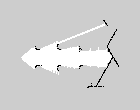
\includegraphics[width=32mm]{img/crop_input.png} &   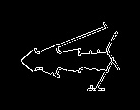
\includegraphics[width=32mm]{img/crop_edges.png} \\
(a) Starting grid & (b) Edge detection \\[6pt]
 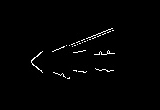
\includegraphics[width=32mm]{img/crop_res.png} &   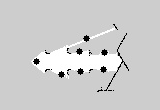
\includegraphics[width=32mm]{img/crop_points.png} \\
(c) Obstacle filtering & (d) Grid with frontiers \\
\end{tabular}
\caption{\textbf{Frontier Detection}}
\label{fig:cv}
\end{figure}
This approach allows the identification of a singular, centroid point for each frontier. In constrast, sampling-based methods would result in the identification of multiple points associated with the same frontier, necessitating additional processes like clustering for consolidation.

After the frontiers identification, the subsequent step involves the allocation of these frontiers to individual robots. In order to do so, we define a reward function $R_{ij}$ for all robot-frontiers $(i,j)$ pairs. This function serves to provide an estimate of the best frontiers for each robot to explore.
As explained in Section \ref{sec:literature_exploration}, most existing methodologies rely on the robot-frontier distance as the sole cost metric. In this work, a new reward function is introduced, which aims at finding a reasonable trade-off between costs associated with the distance and reward in the exploration. The expression is the difference between the information gain and the cost for the robot to reach that frontier:
$$ R_{ij} = I_{j} - C_{ij}$$
The length of contour describing the frontier is introduced as an indicator of the information gain. In this way, exploration of large unknown areas is also promoted, rather than the simple exploitation of nearby, smaller frontiers.
The literature suggests alternative indicators for information gain, such as the percentage of unexplored cells within a defined radius around the frontier point. However, we opt for computational efficiency by avoiding to loop over the grid multiple times. For the same reason, we do not introduce a cost linked to the length of the path to reach the assigned frontier, but rather consider only the Cartesian distance. This design enables the path planning algorithm to be invoked just once, following the frontier-robot assignment.
Heuristics can be applied to the reward calculation, in the sense that we set the reward to -inf if other robots are very close to a frontier (but not assigned to it). 

The assignment strategy follows a greedy policy, in terms of maximizing the reward. At the same time, it is ensured that no more than one robot is assigned to a specific frontier:
%%%% Greedy-Algorithm 
\begin{algorithm}
\caption{Greedy Frontier Assignment}
 \hspace*{\algorithmicindent} \textbf{Input} Robot set $P$, Frontier set $F$, Reward matrix $R$\\
 \hspace*{\algorithmicindent} \textbf{Output} $\alpha_{ij}$  assignment of robot $P_i$ to frontier $F_j$\\
\begin{algorithmic}[]
    \WHILE{$P$ is not empty}

    \IF{$F = $\,\O}
        \STATE Send robots in $P$ to initial position
    \ELSE
    
    \STATE Find $i,j$ = argmax $R_{ij}$ $\forall P_i \in P, \,\forall F_j \in F$
    \STATE $\alpha_{ij}$ = 1
    \ENDIF
    \STATE $P = P \,\backslash\, P_i$, $F = F \,\backslash\, F_j$
    \ENDWHILE{}
\end{algorithmic}
\end{algorithm}
%If the reward is defined well, then a simple greedy assignment strategy can be reasonably effective. There is no need to define a more complex policy, especially if the number of robots is not large.


\subsection{Path Planning}
In this study, we adopt the A* algorithm to address the path planning problem. Sampling-based techniques are particularly advantageous in high-dimensional spaces where the computational demands of grid-based approaches become prohibitively high. In our specific application context, we have access to a 2D grid of moderate size, making graph search methods the most suitable choice.

In the present work we present an enhanced version of the A* algorithm by integrating it with an artificial potential field generated through the Fast Marching Method (FMM) \cite{fast_marching}. 
The Fast Marching Method (FMM) \cite{fast_marching} is a numerical technique widely employed in computational physics and computer science for solving the Eikonal equation, which models the propagation of wavefronts. It returns the distance of a point from obstacles in the path. For this reason, it can be used in various domains, specifically in robotics path planning.

The original A* algorithm makes use of a priority queue to efficiently navigate through the grid. Points are extracted from the priority queue using an heuristic, which represent the total cost of the path until that point. To ensure adequate clearance from walls and obstacles, we introduce the distance computed by the FMM in the heuristic summation (Fig. \ref{fig:costmap}). This modification guides the expansion of grid-search frontiers in a direction that maintains safe distances from obstacles.

\begin{figure}[H]
  \begin{center}
    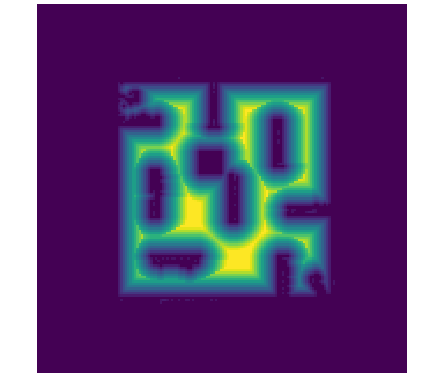
\includegraphics[width=0.4\textwidth]{img/costmap.png}
  \end{center}
  \caption[]{
    \textbf{Fast Marching Method Cost Map.} 
    Lighter squares represent safer regions, darker cells are closer to obstacles. Other robots are also considered as obstacles in the cost map.
  }
  \label{fig:costmap}
\end{figure}

Path tracking and control is achieved by the means of a simple PID pure-pursuit controller \cite{pure_pursuit}, ensuring that the robot follows the path with good flexibility.



\subsection{Point Cloud merging}
\label{sec:point_cl}
For this project work, given the capabilities of RTAB-Map but also the necessity to discover more the process behind map creation, two different approaches to Point Cloud merging where analyzed. 

\begin{algorithm}[b]
\caption{Online mapData Merging} \label{algmapData}
\begin{algorithmic}[1]
\REQUIRE Two RTAB-Map streams of \textit{mapData}, $map\_1$ and $map\_2$ 
\ENSURE Online merged point cloud: $combo\_map\_Data$
    \IF{$timerCallback$}
        \STATE \textbf{Merge maps:}
        \STATE \hspace{0.3cm} Iterate over a subset of nodes in $map\_1$ and process them in shared RTAB-Map.
        \STATE \hspace{0.3cm} Update the length of $map\_1$.

        \STATE \hspace{0.3cm} Iterate over a subset of nodes in $map\_2$ and process them in shared RTAB-Map.
        \STATE \hspace{0.3cm} Update the length of $map\_2$.

        \STATE \hspace{0.3cm} Retrieve poses and constraints from  shared RTAB-Map.
    
        \STATE \textbf{Publish merged map:}
        \STATE \hspace{0.3cm} Retrieve poses and constraints and nodes from shared RTAB-Map.
        \STATE \hspace{0.3cm} Create a new mapData type message
        \STATE \hspace{0.3cm} Publish the new message on the $combo\_map\_Data$ stream
    
    \ENDIF
\end{algorithmic}
\end{algorithm}

The first one, where the complete map is created in \textbf{real-time}, leverages directly the RTAB-Map built in functions and the suggestions given by the community \cite{rtabmapforum}. In this solution, we deploy a collaborative solution based on a hybrid \textit{decentralized} and later \textit{centralized} approach. To obtain this solution, three different instances of RTAB-Map are used: two of them are applied on the creation of two local, individual point cloud maps maps, one on each of the robots. In real time the data coming from these two point clouds is fed in a third dummy instance of RTAB-Map, where the nodes created in the two maps are merged in a sequential manner to obtain a fully merged global map. To obtain this, the requirement is to set the initial poses of the two robots such that the first visual detection is executed on the same object or scenario: this allows for an initial correct loop closure between the two maps and a optimal starting point for the creation of the whole point cloud map. The procedure follows by Algorithm \ref{algmapData}, where the most important steps are outlined. It is important to say that this code is heavily dependant on the libraries created in RTAB-Map: this leads to the creation of \textit{database} (.db) files that can only be read with a softwer connected to RTAB-Map. In order to store directly the point clouds it would be necessary to create a stream of point cloud points directly in .ply or similar file types.

\begin{algorithm}[tbh]
\caption{ICP Registration and offline PC Merging} \label{algICP}
\begin{algorithmic}[1]
\REQUIRE Two point clouds: $PC_1$ and $PC_2$, Maximum Iterations: \textit{max\_iter}
\ENSURE Aligned and merged point cloud: $final\_PC$

\STATE \textbf{tr-ICP Registration:}
    
    \FOR{ $iter$ in range($max\_iter$)}
        \STATE \textbf{Nearest Neighbor Search Using KD-Tree:}
        \STATE \hspace{0.3cm} Find nearest neighbors between $PC_1$ and $PC_2$ using a KD-tree.
        \STATE \hspace{0.3cm} Store a shuffled, partial version of the results in the $idx$ matrix.
    
        \STATE \textbf{Refine the Transformation (ICP Step):}
        \STATE \hspace{0.3cm} Refine the transformation between $PC_1$ and $PC_2$ using nearest neighbor correspondences.
        \STATE \hspace{0.3cm} Compute the transformation matrix $R_T$.
        \STATE \hspace{0.3cm} Apply $R_T$ to $PC_1$ to align it with $PC_2$.
    
    \ENDFOR

\STATE \textbf{ICP Merging Point Clouds:}
    \STATE \hspace{0.3cm} \textbf{Nearest Neighbor Search Using KD-Tree:}
        \STATE \hspace{0.6cm} Find nearest neighbors with KD-tree.
        \STATE \hspace{0.6cm} Store the total results in the $idx$ matrix.
    \STATE \hspace{0.3cm} \textbf{Merging:}
        \STATE \hspace{0.3cm} Copy one point cloud and all of its not neighbors from the other in $final\_PC$
    
\RETURN $final\_PC$
\end{algorithmic}
\end{algorithm}

Given the necessity to depend on RTAB-Map, and given the possible errors of rotation and translation between the two point clouds obtained, an additional algorithm is presented, where the manipulation is executed directly on the point clouds, without the necessity of other software. The second algorithm proposes an offline, post processing of the point clouds generated by the two instances of RTAB-Map, where a ICP algorithm is deployed for the alignment of the two maps and a duplicate point elimination in order to obtain a point cloud map without any redundant point in it. This is crucial to obtain as few points as possible in the point cloud, allowing for better storing and faster manipulation. This is depicted in  Algorithm \ref{algICP}. This algorithm leverages various libraries such as \textit{Eigen} \cite{guennebaud2010eigen} for linear algebra and matrices manipulation and \textit{nanoflann} \cite{blanco2017nanoflann} for KD-tree-based nearest neighbor search. Given these two libraries, the core of the algorithm are ICP and K-Nearest Neighbour (KNN) serach. The ICP algorithm is a common technique in computer vision and robotics for aligning two sets of 3D points. The ICP registration iteratively refines the transformation between the two point clouds, estimating both rotation and translation components. It is based on the definition of the closest points between two maps, and this is done through a KD-tree data structure. KD-trees are used for nearest neighbor search, which is a fundamental operation in point cloud processing. In this code, the KD-tree is built using the 3D spatial coordinates of one of the point clouds, allowing for fast nearest neighbor queries. The KNN functionality comes into play when searching for the nearest neighbors of points from the other point cloud. By performing KNN searches using the KD-tree, the code efficiently identifies candidate corresponding points between the two point clouds. These initial correspondences are then refined through the iterative ICP registration process, ultimately leading to an accurate alignment and merging of the point clouds. KNN is a critical component in finding these initial correspondences, which are essential for the success of the registration algorithm. The incorporation of both KNN search and ICP map reconstruction allows also to avoid overlapping points in the final point cloud, leading to more uniform density in the final merged map, as it can be seen in Figure \ref{fig:example}.


\section{Results}
\label{sec:results}
Simulations are first run on a simpler map to test the system's navigation features, being the assignment of the exploration goal and the generation of a feasible path. Following, a more complex environment is selected to visualize the correctness of the reconstructed point cloud.
We initially deploy two robots in the \textit{Turtlebot3 stage 4} world \cite{turtlebot3-simulation}. The agents are capable of autonomously navigate through the environment, continuously exploring the detected frontiers and updating the global map. In Figure \ref{fig:path}, it can be observed how smooth paths are generated, connecting the robot with the frontier with most reward.

\begin{figure}[h]
  \begin{center}
    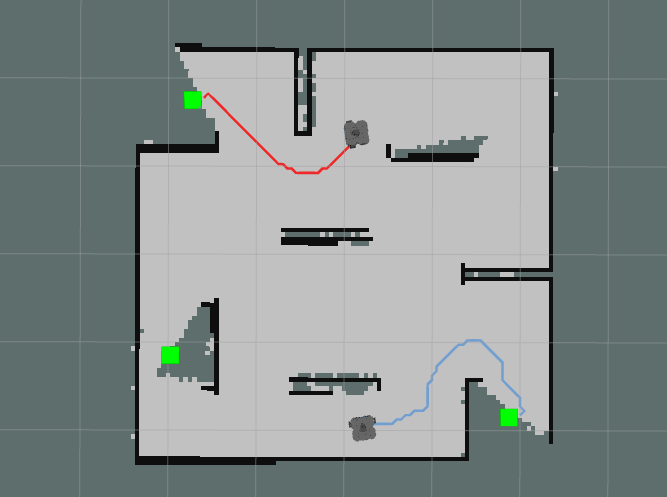
\includegraphics[width=0.4\textwidth]{img/path.png}
  \end{center}
  \caption[]{
    \textbf{Paths generated combining A* with FMM.} 
    Green squares represent the detected frontiers.
  }
  \label{fig:path}
\end{figure}

We now move to analyzing the efficiency of the exploration strategy. We will compare a strategy which uses reward function only based on the distance robot-frontier, and one where the information gain is added.
10 simulations are run with each strategy, and the mean and standard deviation of the explored area overtime are reported. Initial 2D poses for the robots, in terms of (x, y, yaw), are set to $[-0.3, -0.5, \pi/2]$ and $[-1, -0.5, \pi/2]$. The vehicle control policy, in terms of linear and angular acceleration, is kept the same for both strategies.
In Figure \ref{fig:results}, the explored area (in $m^2$) is compared with respect to the time required to map it.
\begin{figure}[b]
  \begin{center}
    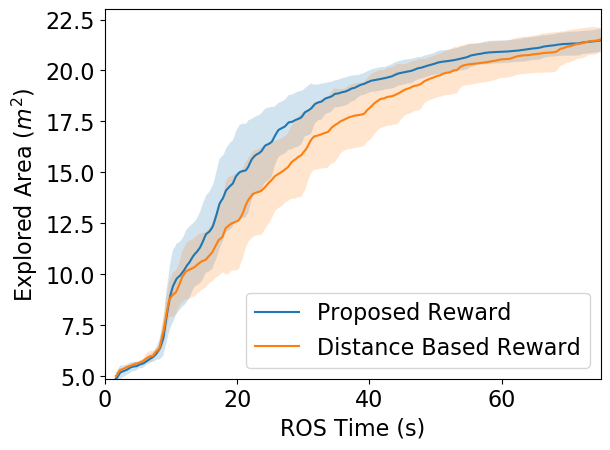
\includegraphics[width=0.49\textwidth]{img/mapping_speed.png}
  \end{center}
  \caption[]{
    \textbf{Exploration Strategy Results.} 
  }
  \label{fig:results}
\end{figure}
As it can be observed, both reward functions typically result in comprehensive map exploration within a similar timeframe. However, the introduction of information gain significantly expedites the initial phases of exploration. Initially, the robot will prioritize large frontiers, leaving smaller areas as unexplored. In this way, it is possible to rapidly obtain a rough version of the map, where most of the macro-regions have been explored. While this behavior proves effective in simpler maps, it may lead to reduced efficiency in more complex environments. For larger spaces, complete exploration may take longer, as nearby frontiers are deprioritized and revisited only much later. Consequently, this approach necessitates fine-tuning of the exploration gain based on the specific map.

Moving forward, we analyze the quality of the point cloud depending on the approaches proposed in the Section \ref{sec:point_cl}.
Regarding the merged point clouds, there is minimal or no difference between the results obtained with the online and offline solutions. This is due to the fact that the initial guess for the initial pose of the robots was accurate, therefore in the end there is minimal or no roto-translation between the two results. The final merged point cloud can be seen in Figure \ref{fig:merged}, where the standard \textit{Home} world from the Turtlebot3 project was used for the simulation \cite{turtlebot3-simulation}. 

\begin{figure}[H]
  \begin{center}
    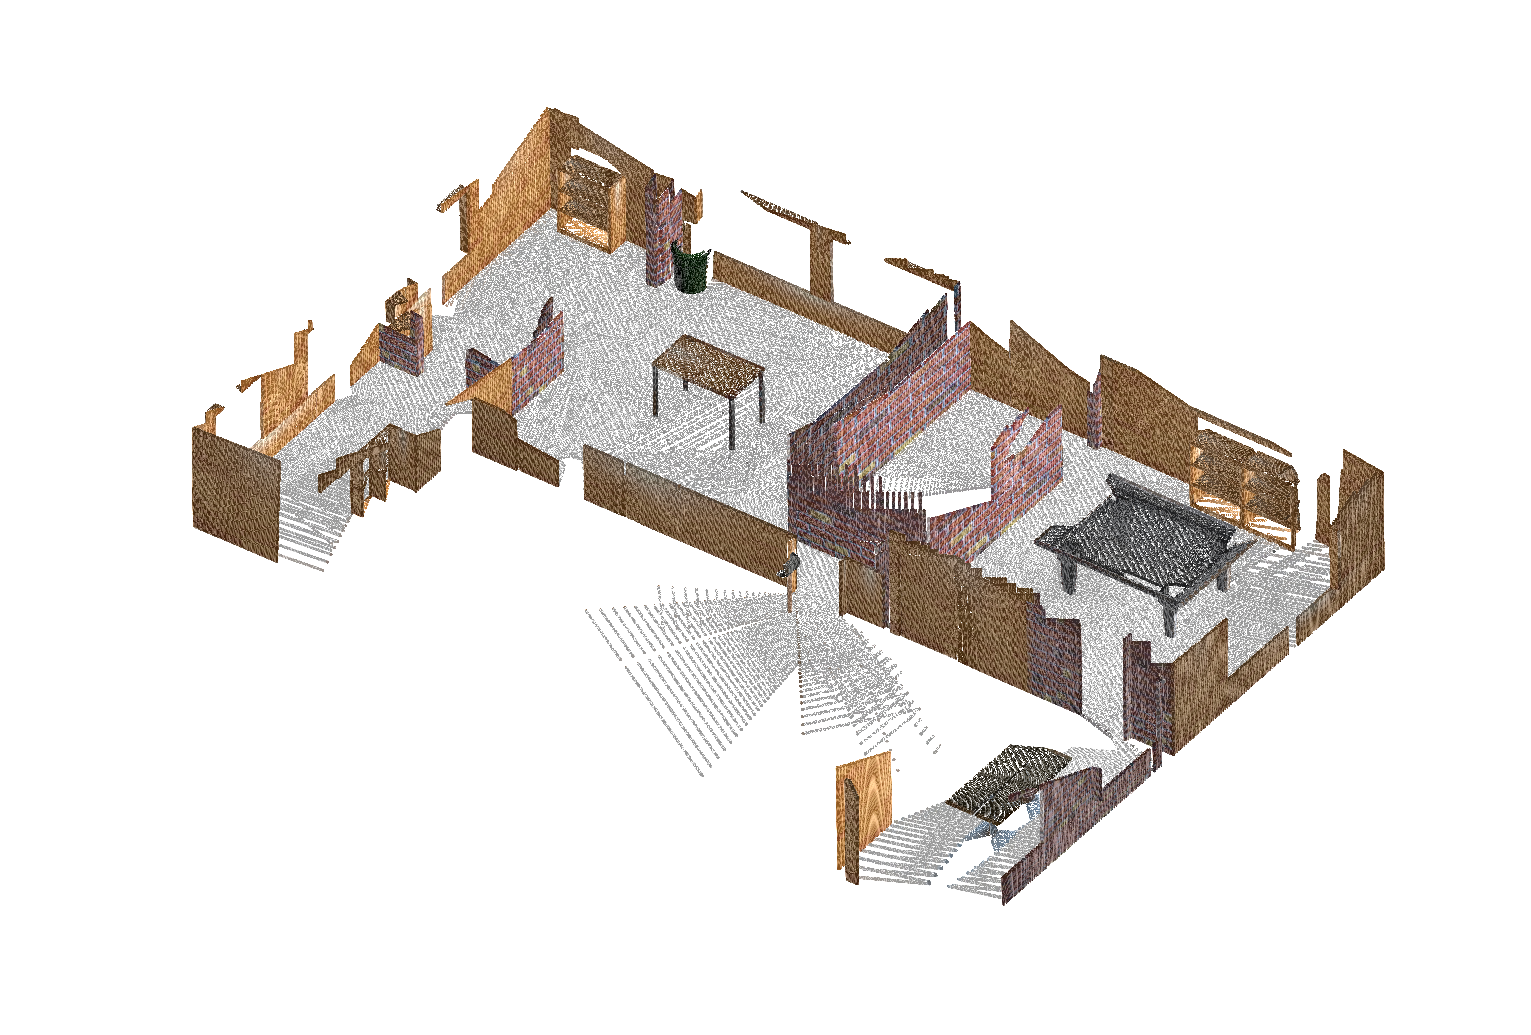
\includegraphics[width=0.49\textwidth]{img/merged.png}
  \end{center}
  \caption[]{
    \textbf{Final merged map} 
  }
  \label{fig:merged}
\end{figure}

Focusing more on the result obtained with the offline algorithm, in Figure \ref{fig:split} it is possible to see the two halves of the merged point cloud, that come from the two instances of RTAB-Map used during the simulation. 

\begin{figure}[H]
  \begin{center}
    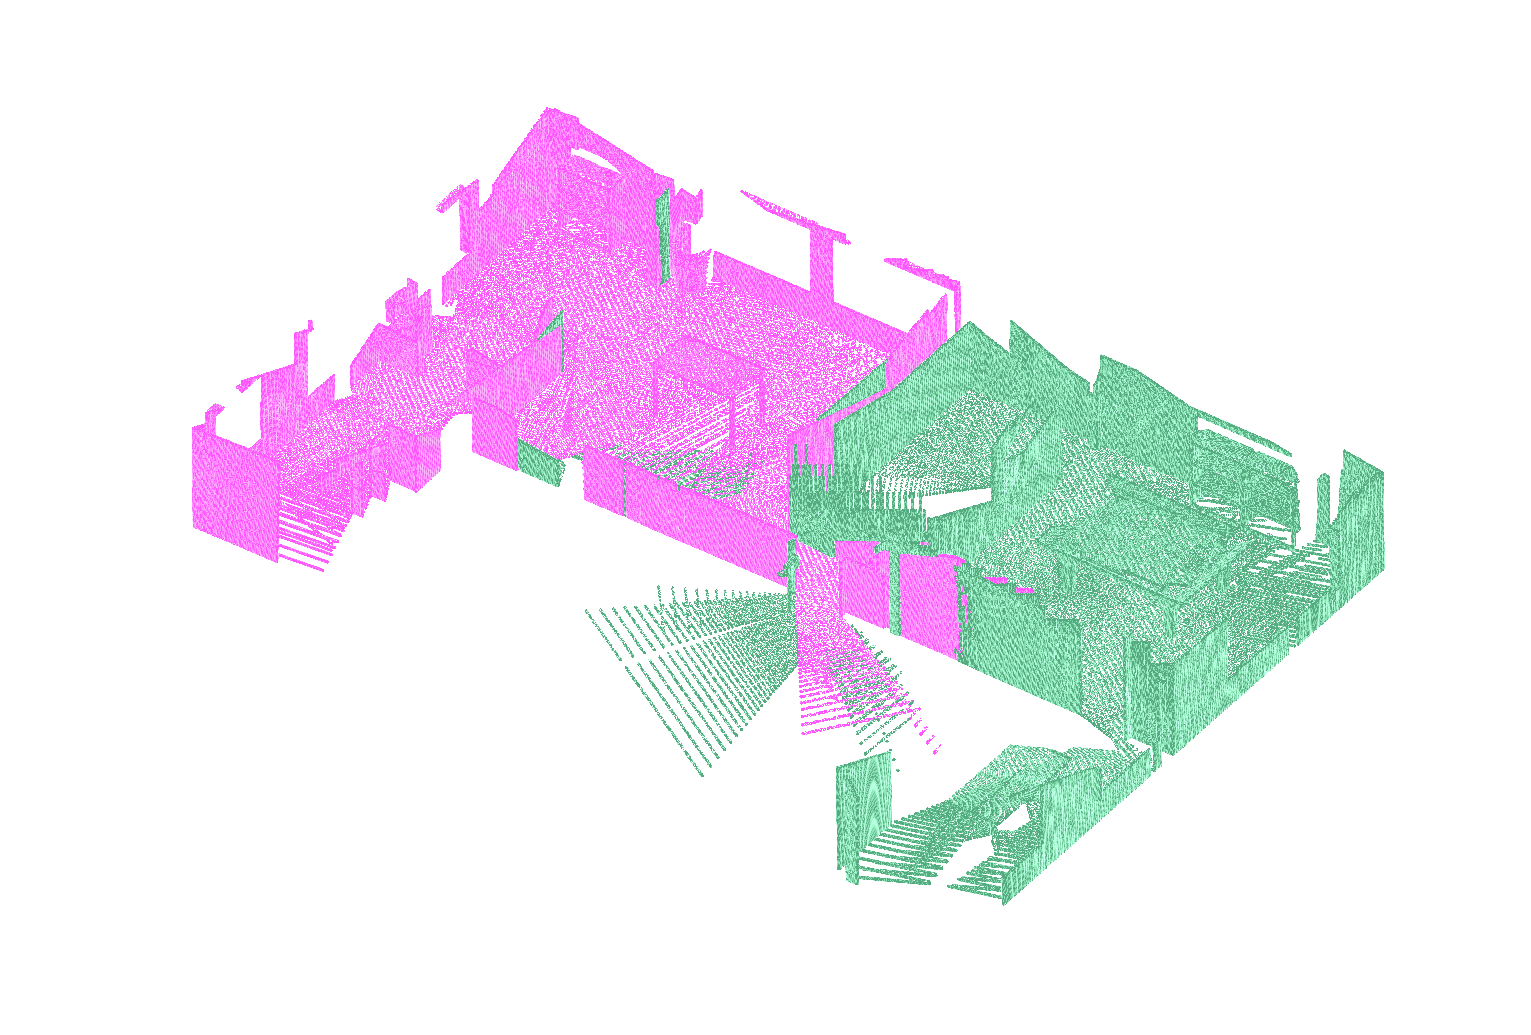
\includegraphics[width=0.49\textwidth]{img/split.png}
  \end{center}
  \caption[]{
    \textbf{Maps merged to form the final map} 
  }
  \label{fig:split}
\end{figure}

Finally, in Figure \ref{fig:example}, it is possible to see how the points shared between the two point clouds are handled by the algorithm. It can be observed that around the pink point there is a empty space, since the approach used in the algorithm \ref{algICP} needs a maximal distance in where the neighbours must be found: these neighbours will be later discarded since they are considered as overlapping, allowing for a final result with less overall points.

\begin{figure}[b]
  \begin{center}
    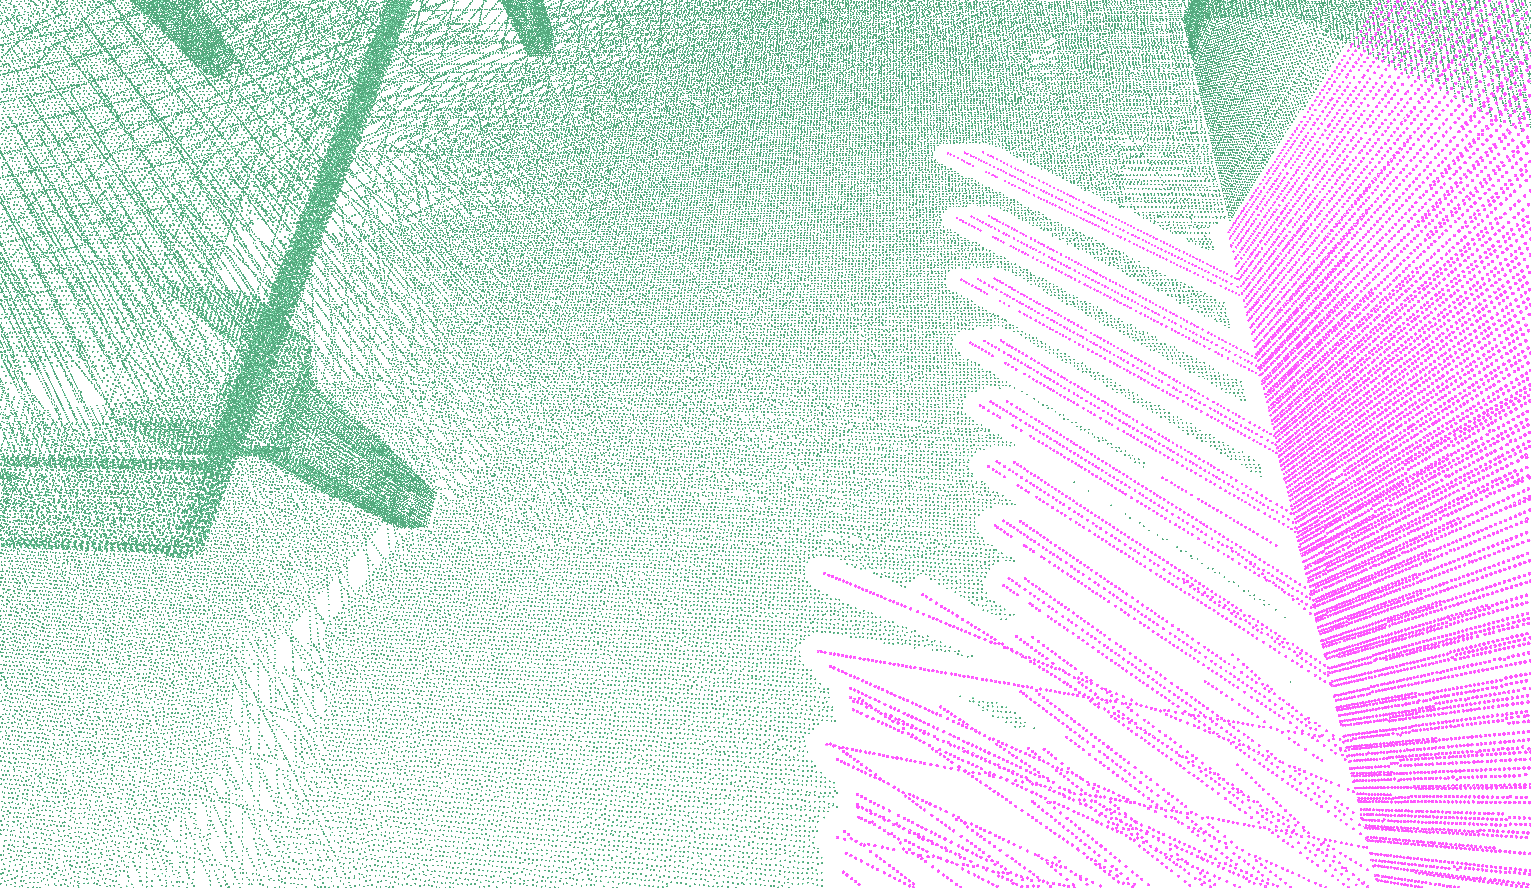
\includegraphics[width=0.49\textwidth]{img/example.png}
  \end{center}
  \caption[]{
    \textbf{Particular on points selection} 
  }
  \label{fig:example}
\end{figure}



%\section{Limitations and future Work}
%Still relatively computationally expensive, but mostly because we deploy RTAB-Map for every robot and the amount of data to be computed in real time comprises all the point clouds generated. Different approaches can optimize this aspect, like density of the point cloud and area mapped at each iteration, but these come at a cost of quality and completeness of the map.  

%Future work:
%\begin{itemize}
%    \item \textbf{Implementation of logic based on qr codes:} the qr codes could be used in a way: on one side they could be used as loop closure triggers, on the second side a logic of navigation could be developed. For the first usage, the qr codes could be put in sections where bottlenecks occur and it is guaranteed that the robots will all visit that section, therefore letting them now to have a best attempt in loop closure in that specific region. For the second usage, this placement could be used as "direction sign" if any knowledge of the map is known a-priori, leading to a better organization of the robots and locations covered
%   \item New reward functions and assignment, non greedy magari.
%    \item " The overall exploration scheme is heavily centralized. A central agent decides which frontier each robot should explore. Centralized coordination scheme represents a single point of failure and requires an additional computation and communication cost " \cite{halscience}. A distributed scheme might work like "each robots computes its cost and bids", so you could have some parallel computation of the cost of the path. If future reward strategies involve a lot of computation for the reward, then it might be the case to adopt a decentralized scheme. For now, with low number of robots and simple reward function, it is best to keep the communication overhead at minimum.
%    \item Find a way to improve the fact that robot cannot map right in front of him
%\end{itemize}
\section{Conclusion}
\label{sec:conclusion}
This work has presented a generic approach for multi-robot exploration and mapping using RGB-D cameras as main sensor. The problem has been tackled by considering its sub-challenges, namely SLAM and point cloud handling, exploration strategy and path planning.

\begin{figure}[H]
  \begin{center}
    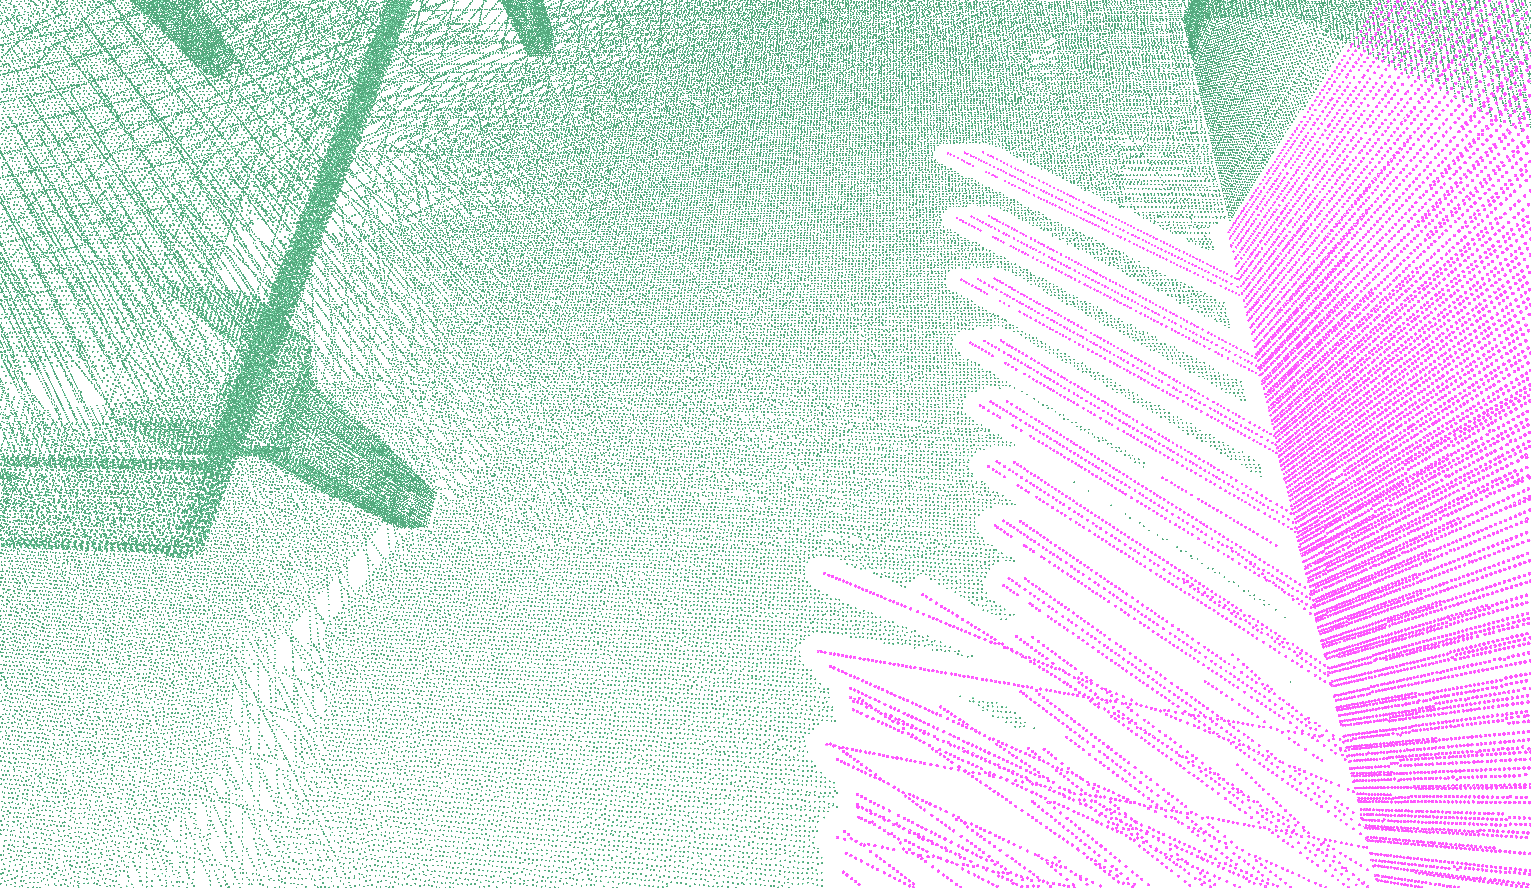
\includegraphics[width=0.49\textwidth]{img/example.png}
  \end{center}
  \caption[]{
    \textbf{Particular on points selection} 
  }
  \label{fig:example}
\end{figure}


Overall, the proposed framework is capable of achieving an accurate mapping, leveraging the capabilities of the RTAB-Map software and point cloud merging algorithms. At the same time, the proposed strategies for exploration and navigation guarantee efficiency and safety in obstacle avoidance.

Future work will focus on testing the system with a larger number of agents, potentially deploying the software on real robots. Any knowledge a-priori of the environment, like QR codes, could be used as loop closure triggers, relieving the software from identifying closures from visual features. In the exploration task, more complex reward functions can be defined and new assignment strategies can be tested. 


%Implementation of logic based on qr codes:} the qr codes could be used in a way: on one side they could be used as loop closure triggers, on the second side a logic of navigation could be developed. For the first usage, the qr codes could be put in sections where bottlenecks occur and it is guaranteed that the robots will all visit that section, therefore letting them now to have a best attempt in loop closure in that specific region. For the second usage, this placement could be used as "direction sign" if any knowledge of the map is known a-priori, leading to a better organization of the robots and locations covered

% Still relatively computationally expensive, but mostly because we deploy RTAB-Map for every robot and the amount of data to be computed in real time comprises all the point clouds generated. Different approaches can optimize this aspect, like density of the point cloud and area mapped at each iteration, but these come at a cost of quality and completeness of the map.  
%New reward functions and assignment, non greedy magari.



\ifCLASSOPTIONcaptionsoff
  \newpage
\fi



\bibliographystyle{./IEEEtran}
\bibliography{references}


\end{document}


